\documentclass[french, 9pt]{article}

%-------------------------------------------------------------------------------
\usepackage[a4paper,top=1cm,bottom=1cm,left=1cm,right=1cm,marginparwidth=0.5cm]{geometry}
\usepackage{amsmath,amsfonts,amssymb,amsthm}
\usepackage[french]{babel}
\usepackage[utf8]{inputenc}
\usepackage[T1]{fontenc}
\usepackage{enumerate}
\usepackage{natbib}
\usepackage{graphicx}
\usepackage{xspace}
\usepackage{color,xcolor}
\usepackage{tikz}
\usepackage{remreset}
\usepackage{url}
\usepackage{boites}
% \usepackage{extsizes} % Permet \documentclass[french, 14pt]{extreport}
% \usepackage[a4paper,top=1cm,bottom=2cm,left=1cm,right=1cm,marginparwidth=.75cm]{geometry}
% \usepackage{minitoc}

\graphicspath{{../Figures/}}
% Environnement
\newtheorem{theorem}{Théorème}
\newtheorem{definition}{Définition}
\newtheorem{lemma}{Lemme}
\newtheorem{proposition}{Proposition}
\newtheorem*{theorem*}{Théorème}
\newtheorem*{definition*}{Définition}
\newtheorem*{proposition*}{Proposition}
\newtheorem*{corollary*}{Corollaire}
\newtheorem*{assumption*}{Hypothèse}
\newtheorem*{algorithm*}{Algorithme}
\newtheorem*{lemma*}{Lemme}
\newtheorem*{remark*}{Remarque}
\newtheorem*{exercise*}{Exercice}
\newtheorem{exercise}{Exercice}
\newcommand{\remark}{\bigskip\noindent\textbf{\textsl{Remarque.}}\xspace}
\newcommand{\remarks}{\bigskip\noindent\textbf{\textsl{Remarques.}}\xspace}
\newcommand{\parSR}[1]{\paragraph*{\textsl{#1}}\xspace}
\renewcommand{\proof}{\bigskip\noindent\underline{\textsl{Démonstration}.}\xspace}
\newcommand{\eproof}{$\blacksquare$}

% Effets, couleurs
\newcommand{\emphase}[1]{\textcolor{red}{#1}}
\newcommand{\demoProp}[1]{\noindent{\textbf{\textsl{Démonstration de la proposition \ref{#1} :}}}}
\newcommand{\itemdot}{\textbullet}

% Moments
\DeclareMathOperator{\Esp}{\mathbb{E}}
\DeclareMathOperator{\diag}{diag}
\DeclareMathOperator{\Cov}{\mathbb{C}ov}
\DeclareMathOperator{\tr}{tr}
\DeclareMathOperator{\Var}{\mathbb{V}}
\let\Pr\relax\DeclareMathOperator{\Pr}{\mathbb{P}}
\renewcommand{\d}{\text{d}}

% R, N, ...
\newcommand{\cst}{\text{cst}}
\newcommand{\Cbb}{\mathbb{C}}
\newcommand{\Ibb}{\mathbb{I}}
\newcommand{\Nbb}{\mathbb{N}}
\newcommand{\Rbb}{\mathbb{R}}
\newcommand{\Zbb}{\mathbb{Z}}

% Indicateurs

% Lois et ensembles
\newcommand{\Acal}{\mathcal{A}}
\newcommand{\Bcal}{\mathcal{B}}
\newcommand{\Ccal}{\mathcal{C}}
\newcommand{\Ecal}{\mathcal{E}}
\newcommand{\Gcal}{\mathcal{G}}
\newcommand{\Ical}{\mathcal{I}}
\newcommand{\Lcal}{\mathcal{L}}
\newcommand{\Mcal}{\mathcal{M}}
\newcommand{\Ncal}{\mathcal{N}}
\newcommand{\Pcal}{\mathcal{P}}
\newcommand{\Rcal}{\mathcal{R}}
\newcommand{\Scal}{\mathcal{S}}
\newcommand{\Ucal}{\mathcal{U}}
\newcommand{\Xcal}{\mathcal{X}}
\newcommand{\Ycal}{\mathcal{Y}}

% Comments
\newcommand{\SR}[2]{\textcolor{gray}{#1}\textcolor{red}{#2}}
\newcommand{\todo}[1]{\textcolor{red}{\`A faire~: {\sl #1}}}
\newcommand{\dessin}[1]{
\begin{center}\framebox{\begin{minipage}{\textwidth}
  \textcolor{purple}{#1}
\end{minipage}}\end{center}
\bigskip
}
\newcommand{\progres}[1]{
\begin{center}\framebox{\begin{minipage}{\textwidth}
  \textcolor{blue}{{\sl #1}}
\end{minipage}}\end{center}
\bigskip
}
\newcommand{\solution}[1]{
\begin{center}\framebox{\begin{minipage}{\textwidth}
  \noindent{\sl Solution :}
  #1
\end{minipage}}\end{center}
\bigskip
}
% \newcommand{\exemple}[1]{
% \begin{center}\framebox{\begin{minipage}{\textwidth}
%   \parSR{Exemple.}
%   #1
% \end{minipage}}\end{center}
% \bigskip
% }
\newcommand{\exemple}[1]{
\begin{breakbox}
  \parSR{Exemple.}
  #1
\end{breakbox}
\bigskip
}

\newcommand{\SRcorrect}[2]{\textcolor{gray}{#1}\textcolor{blue}{#2}}
\newcommand{\SRcomment}[1]{\textcolor{blue}{[{\sl SR: #1}]}}



% Section numbering
\usepackage{chngcntr}
\renewcommand{\thepart}{\Roman{part}}
% \counterwithout{section}{part}
\setcounter{secnumdepth}{3}
\setcounter{tocdepth}{1}

% Proposition numbering
\renewcommand{\subsubsection}{\section}
% \numberwithin{exercise}{section}
% \numberwithin{equation}{section}

% Suppression des solutions
\renewcommand{\solution}[1]{}

\newcommand{\alglin}{/home/robin/ENSEIGN/Cours/MathBiologie/L3-ENS-Math1/Exercices/AlgLin}
\newcommand{\multivar}{/home/robin/ENSEIGN/Cours/MathBiologie/L3-ENS-Math1/Exercices/MultiVar}
\newcommand{\equadiff}{/home/robin/ENSEIGN/Cours/MathBiologie/L3-ENS-Math1/Exercices/EquaDiff}
\newcommand{\probas}{/home/robin/ENSEIGN/Cours/MathBiologie/L3-ENS-Math1/Exercices/Probas}


% %-------------------------------------------------------------------------------
% %-------------------------------------------------------------------------------
% \title{\Huge{Ce qu'un biologiste doit savoir en mathématiques}}
% \author{SR d'après \cite{Lam20} : Annexes}
% \date{\today}


\title{}

%-------------------------------------------------------------------------------
%-------------------------------------------------------------------------------
\begin{document}
%-------------------------------------------------------------------------------
%-------------------------------------------------------------------------------

\begin{centering}
  \footnotesize{\sc École Normale Supérieure de Paris} 
  
  \bigskip
  \footnotesize{\sc Licence de Biologie L3}
  
  \bigskip
  \footnotesize{\sc Année 2022–23}
  
  \bigskip
  {\bf Mathématiques I : ce qu’un biologiste ne doit pas ignorer} 
  
  \bigskip
  {\sc Examen}
  
\end{centering}

\bigskip
L'épreuve dure 2 heures. 
Les notes de cours individuelles sont autorisées.
L’usage de tout appareil électronique est interdit à l’exception d’une calculatrice.

%-------------------------------------------------------------------------------
% \section{Algèbre linéaire}
%-------------------------------------------------------------------------------
\subsubsection{Dynamique d'une population de Leslie}
%-------------------------------------------------------------------------------

% Cf exercice 5 AL

On considère une population structurée en $n$ classes d'âge. Pour $1 \leq i \leq n$, on note $x_k(t)$ le nombre d'individus de la classe $k$ à la génération $t$ et $x(t) = [x_1(t) \dots x_n(t)]^\top$ le vecteur décrivant l'ensemble de la population à cette même génération. On suppose que l'évolution de cette population est régit par la récurrence
\begin{equation} \label{eq:recurrenceLeslie}
  x(t+1) = A x(t)
\end{equation}
où $A$ est la matrice de Leslie
$$
A = \left[\begin{array}{cccccc}
            f_1 & f_2 & \cdots  & \cdots & f_n \\
            s_1 & 0 & \cdots  & \cdots & 0 \\
            0 & \ddots  & \ddots & & \vdots \\
            \vdots & \ddots & \ddots & \ddots & \vdots \\
            0 & \cdots & 0 & s_{n-1} & 0 \\
          \end{array}\right]
$$
où tous les coefficients $f_i$ et $s_i$ sont supposés strictement positifs. On note de plus
$$
\ell_1 = 1 \qquad \text{et} \qquad 
\ell_k = \prod_{i=1}^{k-1} s_i \quad \text{pour $2 \leq k \leq n$}.
$$

\begin{enumerate}
  \item Interprêter les coefficients $f_i$ et $s_i$.
  \solution{$f_i$ est le taux de fertilité de la classe $i$ (qui alimente la classe 1). $S_i$ est le taux de survie de la classe $i$ (qui alimente la classe $i+1$).}
  %
  \item Soient $B_{k1} \in \Mcal_{k-1}$, $B_{k2} \in \Mcal_{n-k}$ définies par :
  $$
  B_{k1} = \left[\begin{array}{cccc}
            s_1 & -\lambda & &  \\
            & \ddots & \ddots & \\
            & & \ddots & -\lambda \\
            & & & s_{k-1}
          \end{array}\right], \qquad
  B_{k2} = \left[\begin{array}{cccc}
            -\lambda & & & \\
            s_{k+1} & \ddots & & \\
            & \ddots & \ddots & \\
            & & s_{n-1} & -\lambda
          \end{array}\right].
  $$
  En notant $0_{p,q}$ la matrice $p \times q$ dont tous les éléments sont nuls, calculer le déterminant de la matrice $B_k \in \Mcal_{n-1}$ :
  $$
  B_k = \left[\begin{array}{cc}
            B_{k1} & 0_{k-1, n-k} \\
            0_{n-k, k-1} & B_{k2}
          \end{array}\right].
  $$
  \solution{On utilise le calcul du déterminant par bloc pour obtenir
  $$
  |B| = |B_{k1}| \times |B_{k2}|
  $$
  et on remarque que, puisque $B_{k1}$ et $B_{k2}$ sont respectivement triangulaires supérieure et inférieure, leurs déterminants sont égaux au produit de leurs termes diagonaux, soit
  $$
  |B_{k1}| = \ell_k, \qquad |B_{k2}| = (-\lambda)^{n-k}.
  $$
  }
  %
  \item Montrer que le polynôme caractéristique de $A$ est
  $$
  P_A(\lambda) = (f_1 - \lambda) (-\lambda)^{n-1} + \sum_{k=2}^{n} (-1)^{k-1} f_k \ell_k (-\lambda)^{n-k}.
  $$
  \solution{Les termes successifs du développement du déterminant 
  $$
  |A - \lambda I| 
  = \left|\begin{array}{cccccc}
            f_1-\lambda & f_2 & \cdots  & \cdots & f_n \\
            s_1 & -\lambda & 0  & \cdots & 0 \\
            0 & s_2 & \ddots & \ddots & \vdots \\
            \vdots & \vdots & \ddots & \ddots & 0 \\
            0 & \cdots & 0 & s_{n-1} & -\lambda \\
          \end{array}\right|
  $$ 
  par rapport à la première ligne sont
  \begin{align*}
  (f_1 - \lambda) |B_1| & = (f_1-\lambda) (-\lambda^{n-1}), &
  - f_2 |B_2| & = -f_2 s_1 (-\lambda)^{n-2}, \\
  f_3 |B_3| & = f_3 s_1 s_2 (-\lambda)^{n-3}, & 
  -f_4 |B_4| & = -f_4 s_1 s_2 s_3 (-\lambda)^{n-4}, \qquad \dots
  \end{align*}
  }
  %
  \item En déduire que la plus grande valeur propre en module $\lambda_1$ de la matrice $A$ vérifie
  $$
  \sum_{k=1}^n \ell_k f_k \lambda_1^{-k} = 1.
  $$
  \solution{Toutes les valeurs propres, dont $\lambda_1$, sont solutions de $P_A(\lambda) = 0$, soit
  \begin{align*}
  (f_1 - \lambda) (-\lambda)^{n-1} + \sum_{k=2}^{n} (-1)^{k-1} f_k \ell_k (-\lambda)^{n-k} & = 0 \\
  \Leftrightarrow \qquad \sum_{k=1}^n (-1)^{k-1} f_k \ell_k (-\lambda)^{n-k} & = (-\lambda)^{n-1} & 
  \Leftrightarrow \qquad \sum_{k=1}^n f_k \ell_k \lambda^k & = 1.
  \end{align*}
  }
\end{enumerate}

On s'intéresse maintenant aux vecteurs propres à gauche et à droite de la matrice $A$. On note 
$$
a = \sum_{k=1}^n \ell_k \lambda_1^{-k}, \qquad
b = \sum_{k=1}^n k \ell_k f_k \lambda_1^{-k}.
$$
\begin{enumerate}
  \setcounter{enumi}{4}
  \item Montrer que le vecteur $v$ de coordonnées
  $$
  v_k = \frac1a \ell_k \lambda_1^{-k}, \qquad 1 \leq k \leq n,
  $$
  est un vecteur propre à droite de $A$ associé à la valeur propre $\lambda_1$.
  \solution{Soit le vecteur $w = Av$. Ses coordonnées sont
  \begin{align*}
    w_1 & = \sum_{k=1}^n f_k v_k = \frac1a \sum_{k=1}^n f_k \ell_k \lambda_1^{-k} = \frac1a = \lambda_1 v_1, \\
    w_k & = s_{k-1} v_{k-1} = \frac1a s_{k-1} \ell_{k-1} \lambda_1^{-k+1}  = \frac1a \ell_k \lambda_1^{-k+1} = \lambda_1 v_k, \qquad \text{pour $2 \leq k \leq n$}.
  \end{align*}
  }
  \item Montrer que le vecteur $u$ de coordonnées
  $$
  u_k = \frac1{b v_k} \sum_{j=k}^n \ell_j f_j \lambda_1^{-j}, \qquad 1 \leq k \leq n,
  $$
  est un vecteur propre à gauche de $A$ associé à la valeur propre $\lambda_1$.
  \solution{Soit le vecteur $w^\top = u^\top A$. On a
  $$
  w_n = f_n u_1
    = f_n \frac{a \lambda_1}b \sum_{j=1}^n \ell_j f_j \lambda_1^{-j}
    = f_n \frac{a \lambda_1}b
  $$
  or
  $$
  u_n = \frac{\ell_n f_n \lambda_1^{-n}}{b v_n} = \frac{a f_n}{b}, 
  \qquad \text{donc} \quad w_n = \lambda_1 u_n.
  $$
  De plus, pour $1 \leq k \leq n-1$, on a
  \begin{align*}
    w_k & = f_k u_1 + s_k u_{k+1} 
    = f_k \frac{a \lambda_1}{b} \sum_{j=1}^n \ell_j f_j \lambda_1^{-j} + s_k \frac{a \lambda_1^{k+1}}{b \ell_{k+1}} \sum_{j=k+1}^n \ell_j f_j \lambda_1^{-j} \\
    & = \frac{a \lambda_1^{k+1}}{b \ell_k} \left(f_k \ell_k \lambda_1^{-k} + \sum_{j=k+1}^n \ell_j f_j \lambda_1^{-j}\right)
    = \lambda_1 \frac{a \lambda_1^k}{b \ell_k} \sum_{j=k}^n \ell_j f_j \lambda_1^{-j}
    = \lambda_1 u_k.
  \end{align*}}
\end{enumerate}

On s'intéresse enfin au comportement asymptotique du vecteur $x(t)$ décrivant la composition de la population au bout de $t$ générations.
\begin{enumerate}
  \setcounter{enumi}{6}
  \item Calculer $\sum_{k=1}^n v_k$ et $\sum_{k=1}^n v_k u_k$.
  \solution{On a
  \begin{align*}
    \sum_{k=1}^n v_k 
      & = \frac1a \sum_{k=1}^n \ell_k \lambda_i^{-k} = 1 \\
    \sum_{k=1}^n v_k u_k 
      & = \frac1b \sum_{k=1}^n \sum_{j=k}^n \ell_j f_j \lambda_1^{-j}
      = \frac1b \sum_{k=1}^n k \ell_k f_k \lambda_1^{-k} = 1.
  \end{align*}}
  \item Partant d'un vecteur de composition initial $x(0)$, quel est le comportement asymptotique de $x(t)$ quand $t$ tend vers l'infini ?
  \solution{La récurrence \eqref{eq:recurrenceLeslie} implique que $x(t) = A^t x(0)$. De plus, le théorème de Perron-Frobénius nous assure que $\lim_{t \to \infty} \lambda_1^{-t} A^t = v u^\top$. On a donc
  $$
  \lim_{t \to \infty} \lambda_1^{-t} x(t) 
  = \lim_{t \to \infty} \lambda_1^{-t} A^t x_0(t)
  = v u^\top x(0) = \left(u^\top x(0)\right) v
  $$
  soit $x(t) \approx c_0 \lambda_1^t v$, avec $c_0 = u^\top x(0)$.
  \begin{itemize}
   \item La taille totale de la population évolue asymptotiquement comme $\lambda_1^n$. 
   \item La composition asymptotique relative de la population est donnée par les coordonnées du vecteur $v$ (qui somment à 1). 
   \item Le produit scalaire $c_0$ indique comment les effectifs initiaux $x_k(0)$ contribuent respectivement (à proportion de $u_k$) à la taille asymptotique de la population.
  \end{itemize}}
\end{enumerate}


%-------------------------------------------------------------------------------
% \section{Fonction de plusieurs variables}
%-------------------------------------------------------------------------------
\subsubsection{Application linéaire tangente à une forme quadratique} 
%-------------------------------------------------------------------------------

On considère une matrice $A \in \Mcal_n$ symétrique, un vecteur $v \in \Rbb^n$ et la fonction 
$$
\begin{array}{rlll}
  f : & \Rbb^n & \mapsto & \Rbb \\
  & x & \to & f(x) = x^\top A x + v^\top x.
\end{array}
$$

\begin{enumerate}
  \item Montrer qu'il existe un vecteur $g(x) \in \Rbb^n$, qu'on précisera, tel que l'application linéaire tangente à $f$ en $x$ s'écrit
  $$
  \begin{array}{rlll}
    D_xf : & \Rbb^n & \mapsto & \Rbb^n \\
    & h & \to & D_xf(h) = g(x)^\top h.
  \end{array}
  $$
  \solution{On écrit
  \begin{align*}
    f(x+h) 
    & = (x+h)^\top A (x+h) + v^\top (x+h)
    = f(x) + x^\top A h + h^\top A x + h^\top A h + v^\top h \\
    & = f(x) + (2 x^\top A + v^\top) h + h^\top A h
  \end{align*}
  puisque $x^\top A h = h^\top A x$. On remarque alors que $h^\top A h = o(\|h\|)$ pour conclure que, puisque $A$ est symétrique, l'application linéaire tangent $D_x f$ s'écrit bien
  $$
  D_xf(h) = g(x)^\top h
  \qquad \text{avec} \quad
  g(x) = 2 A x + v.
  $$}
  \item En supposant que $A$ est inversible, déterminer le point stationnaire $x^*$ où $g(x)$ s'annule.
  \solution{En supposant $A$ inversible, on a
  $$
  g(x^*) = 0
  \qquad \Leftrightarrow \qquad
  2 A x^* + v = 0
  \qquad \Leftrightarrow \qquad
  x^* = - \frac12 A^{-1} v.
  $$}
  \item Donner une condition sur$A$ pour que $A$ soit un minimum local. (On pourra calculer la matrice hessienne de $A$.)
  \solution{La matrice hessienne de l'application $f$ en tout point $x$ vaut $H_x = 2 A$ (il suffit de déterminer l'application linéaire tangente à $g(x)$).
  $x^*$ est donc un minimum ssi $A$ est strictement définie négative}
  \item Discuter l'utilité de l'hypothèse selon laquelle $A$ est symétrique.
  \solution{On peut décomposer $A$ en ses parties symétrique $S$ et anti-symétrique $T$ : 
  $$
  S = \frac12(A + A^\top), \qquad 
  T = \frac12(A - A^\top), \qquad 
  \Rightarrow \quad
  A = S + T
  $$
  et remarquer que
  $$
  f(x) 
  = x^\top A x + v^\top x
  = x^\top S x + \frac12 \underset{=0}{\underbrace{(x^\top A x - x^\top A^\top x)}} + v^\top x,  
  $$
  c'est-à-dire que seulle la partie symétrique de $A$ contribue à la fonction Ode $f$.}
\end{enumerate}




%-------------------------------------------------------------------------------
% \section{Systèmes dynamiques}
%-------------------------------------------------------------------------------
\subsubsection{Système différentiel d'ordre trois} 
%-------------------------------------------------------------------------------

On considère l'équation différentielle ordinaire non-linéaire
\begin{equation} \label{eq:L3BioSUTD2E2}
\dot x = f(x) = -x^3 + 7x^2 - 14x + 8.
\end{equation}
% dans laquelle $x$ désigne la concentration d'un métabolite : \eqref{eq:L3BioSUTD2E2} modélisant l'ensemble des réactions biochimiques impliquées dans la production/dégradation de ce métabolite.

\begin{enumerate}
  \item Déterminer l'ensemble des points stationnaires de \eqref{eq:L3BioSUTD2E2}.
  \solution{On cherche les raçines de $f(x)$. 1 est une racine évidente, et, en déterminant les raçines de $x^2 - 6x + 8$, on voit que $f(x)$ se factorise en
  \begin{align*}
    f(x) & = (x-1) (x^2 - 6x + 8) = (x-1) (x - 2) (x - 4). 
  \end{align*}
  Les points stationnaires sont donc $x^*_1 = 1$, $x^*_2 = 2$ et $x^*_3 = 4$.}
  \item \'Etudier la stabilité de chacun de ces points stationnaires.
  \solution{On calcule
  $$
  f'(x) = -3 x^2 + 14x -15
  $$
  et on conclue 
  \begin{align*}
    f'(x^*_1) & = -3 < 0 & \Rightarrow \quad x^*_1 & = 1 \text{ est stable}, \\ 
    f'(x^*_2) & = + 2 > 0 & \Rightarrow \quad x^*_2 & = 2 \text{ est instable}, \\ 
    f'(x^*_3) & = -6 < 0 & \Rightarrow \quad x^*_3 & = 4 \text{ est stable}. 
  \end{align*}}
  \item Tracer le diagramme de stabilité du système.
  \solution{$$
  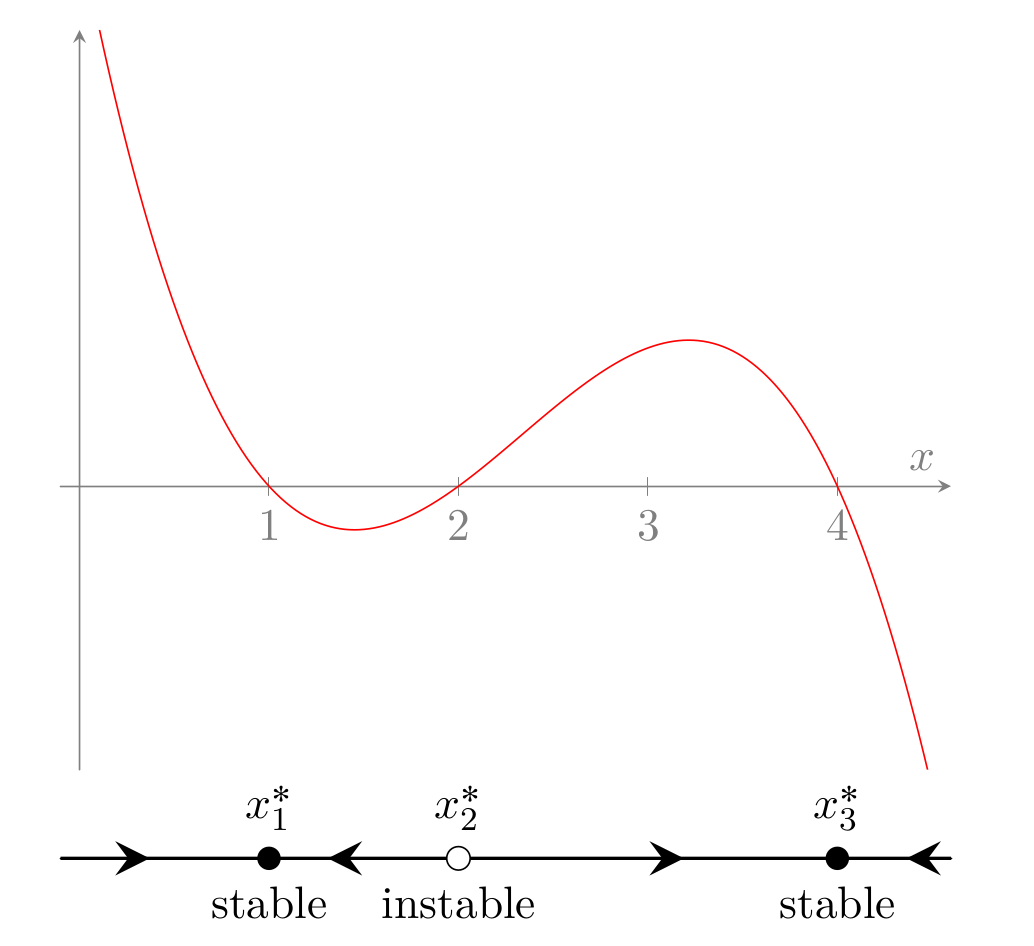
\includegraphics[width=.4\textwidth]{L3bioSU-TD2exo2}
  $$}
  \item D'un point de vue du comportement du système, quels sont les rôles respectifs de chacun des points stationnaires.
  \solution{
  \begin{itemize}
   \item $x^*_1$ et $x^*_3$ sont des équilibre stables et attracteurs vers lesquels le système tend. On perle de bistabilité.
   \item $x^*_2$ est le point critique (stationnaire mais répulsif) : la position de $x(0$ par rapport à $x^*_2$ détermine l'état final du système.
  \end{itemize}}
\end{enumerate}


%-------------------------------------------------------------------------------
% \section{Probabilités}
%-------------------------------------------------------------------------------
\subsubsection{Chaîne de Markov à deux états absorbants}
%-------------------------------------------------------------------------------

On considère une chaîne de Markov $(X_n)_{n \geq 0}$ prenant ses valeurs dans $\{0, \dots \ell\}$, et on note $p_{i, j}$ la probabilité de transition de de l'état $i$ vers l'état $j$. On suppose que 
$$
p_{0, 0} = p_{\ell, \ell} = 1 
$$
et que, pour tout $1 \leq i, j \leq \ell-1$, 
$$
p_{i, 0} = a > 0, \qquad p_{i, \ell} = b > 0, \qquad p_{i, j} \geq 0.
$$
On note de plus $T_{i, j}$ le temps d'atteinte de l'état $j$ à partir de l'état $i$:
$$
T_{i, j} = \min\{n: X_n = j \mid X_0 = i\}.
$$

\begin{enumerate}
  \item Donner la matrice de transition et tracer le graphe de transition de cette chaîne de Markov.
  \solution{
  $$
  P = \left(\begin{array}{c|ccc|c}
              1 & 0 & \cdots & 0 & 0 \\
              \hline
              a & p_{2, 2} & \cdots & p_{2, a-1} & b \\
              \vdots & \vdots &  & \vdots & \vdots \\
              a & p_{a-1, 2} & \cdots & p_{a-1, a-1} & b \\
              \hline
              0 & 0 & \cdots & 0 & 1
          \end{array}\right).
  $$}
  \item Quelles sont les classes de communication de cette chaîne ? Donner leur nature. Quels sont les comportements asymptotiques possibles de cette chaîne ?
  \solution{Les classes de communications sont 
  $$
  C_1 = \{0\}, \qquad C_2 = \{1, \dots, \ell-1\}, \qquad C_3 = \{\ell\}.
  $$
  $C_1$ et $C_3$ sont absorbantes, $C_2$ est transiente. La chaîne finit nécessairement par être absorbé en 0 ou $\ell$.}
  \item Soit $1 \leq i \leq \ell-1$, donner la probabilité que $X_{n+1} \in \{1, \dots \ell-1\}$ sachant que $X_n = i$.
  \solution{Pour tout $1 \leq i \leq \ell-1$, on a $p_{i, 0} = a$ et $p_{i, \ell} = b$, donc
  $$
  \Pr\{1 \leq X_{n+1} \leq \ell-1 \mid X_n = i\}
  = \Pr\{X_{n+1} \neq 0 \text{ et } X_{n+1} \neq \ell\}
  = 1 -(a+b).
  $$}
  \item En déduire que, pour $1 \leq i \leq \ell-1$, en notant $c = a + b$, 
  $$
  \Pr\{T_{i, 0} = n\} = a (1 - c)^{n-1}, \qquad
  \Pr\{T_{i, \ell} = n\} = b (1 - c)^{n-1}.
  $$
  \solution{A chaque pas de temps, partant d'un état $1 \leq i \leq \ell-1$, la chaîne reste dans $\{1, \dots, \ell-1\}$ avec probabilité $1 - a - b = 1 - c$ et passe dans l'état 0 avec probabilité $a$. Pour atteindre l'état 0 depuis l'état $i$ en $n$ étapes, la chaîne doit rester $n-1$ fois dans $\{1, \dots, \ell-1\}$ (avec probabilité $(1-c)^{n-1}$) puis passer en 0 (avec probabilité $a$). \\
  L'autre résultat s'obtient par symétrie}
  \item Pour $1 \leq i \leq \ell-1$, on note maintenant $T_i$ le temps d’absorption (en 0 ou en $\ell$) : 
  $$
  T_i = \min(T_{i, 0}, T_{i, \ell}).
  $$
  Montrer que $T_i$ suit une loi géométrique $\Gcal(c)$ : $\Pr\{T_i = n\} = c (1 - c)^{n-1}$. \\
  En déduire son espérance.
  \solution{Il suffit de remarquer que l'événement d'absorption au temps $n$ s'écrit
  $$
  \{X_n \in \{0, \ell\}, X_0 = i\} = \{X_n = 0, X_0 = i\} \cup \{X_n = \ell, X_0 = i\}
  $$
  pour en déduire que 
  $$
  \Pr\{T_i = n\} = \Pr\{T_{i, 0} = n\} + \Pr\{T_{i, \ell} = n\} = (a + b) (1 - c)^{n-1}.
  $$
  De plus, en se souvenant que 
  $$
  \sum_{n \geq 1} n x^{n-1} 
  = \partial_x \sum_{n \geq 0} x^n 
  = \partial_x \frac{1}{1 - x}
  = (1 - x)^{-2}, 
  $$
  on obtient
  $$
  \Esp T_i = \sum_{n \geq 1} n c (1 - c)^{n-1} = c (1 - (1-c))^{-2} = 1/c.
  $$}
%   \item Montrer que, pour $1 \leq i \leq \ell-1$, 
%   $$
%   \Pr\{T_{i, 0} < n\} = \frac{a [1 - (1 - c)^{n-1}]}{c}.
%   $$
%   \solution{
%   \begin{align*}
%   \Pr\{T_{i, 0} < n\} 
%   & = \sum_{m =1}^{n-1} \Pr\{T_{i, 0} = m \} 
%   = a \sum_{m = 1}^{n-1} (1 - c)^{m-1} \\
%   & = \frac{a [1 - (1 - c)^{n-1}]}{1 - (1 - c)} 
%   = \frac{a [1 - (1 - c)^{n-1}]}{c}.
%   \end{align*}}
  \item Pour $1 \leq i \leq \ell-1$, calculer la probabilité que, partant de $X_0 = i$ la chaîne de Markov atteigne l'état 0 avant l'état $\ell$.
  \solution{La chaîne atteint 0 avant $\ell$ ssi $T_{i, 0} = T_i$. On remarque que, pour tout $n \geq 1$, on a
  $$
  \Pr\{T_{i, 0} = n \mid T_i = n\}
  = \frac{\Pr\{T_{i, 0} = n, T_i = n\}}{\Pr\{T_i = n\} }
  = \frac{\Pr\{T_{i, 0} = n\}}{\Pr\{T_i = n\}}
  = \frac{a}c.
  $$
  On a donc
  $$
  \Pr\{T_{i, 0} = T_i\}
  = \sum_{n \geq 1} \Pr\{T_{i, 0} = n \mid T_i = n\} \Pr\{T_i = n\} 
  = \sum_{n \geq 1} \frac{a}c \Pr\{T_i = n\}
  = \frac{a}c.
  $$}
  \item Combien valent les espérances respectives de $T_{i, 0}$ et $T_{i, \ell}$ pour $1 \leq i \leq \ell-1$ ?
  \solution{Puisque $a > 0$ et $b > 0$, chacun des deux états absorbants peut ne jamais être atteint : 
  \begin{align*}
  \Pr\{T_{i, 0} & = +\infty\} = \Pr\{T_i = T_{i, \ell}\} = b/c > 0, \\
  \text{et} \qquad
  \Pr\{T_{i, \ell} & = +\infty\} = \Pr\{T_i = T_{i, 0}\} = a/c > 0
  \end{align*}
  donc
  $$
  \Esp T_{i, 0} = \Esp T_{i, \ell} = + \infty.
  $$}
\end{enumerate}



%-------------------------------------------------------------------------------
%-------------------------------------------------------------------------------
\end{document}
%-------------------------------------------------------------------------------
%-------------------------------------------------------------------------------


